\begin{enumerate}
\item Find the coordinates of the point which divides the join of $(-1,7)$ and $(4,-3)$ in the ratio 2:3.
\item Find the coordinates of the points of trisection of the line segment joining $(4,-1)$ and $(-2,3)$.
\item To conduct Sports Day activities, in your rectangular shaped school ground ABCD, lines have been drawn with chalk powder at a distance of 1m each. $100$ flower pots have been placed at a distance of 1m from each other along AD, as shown in \figref{fig:7.12}. Niharika runs $\frac {1}{4}th$ distance AD on the 2nd line and posts a green flag. Preet runs $\frac {1}{5}th$ the distance AD on the eighth line and posts a red flag. What is the distance between both the flags? If Rashmi has to post a blue flag exactly halfway between the line segment joining the two flags, where should she post her flag?
\begin{figure}[ht]
\centering
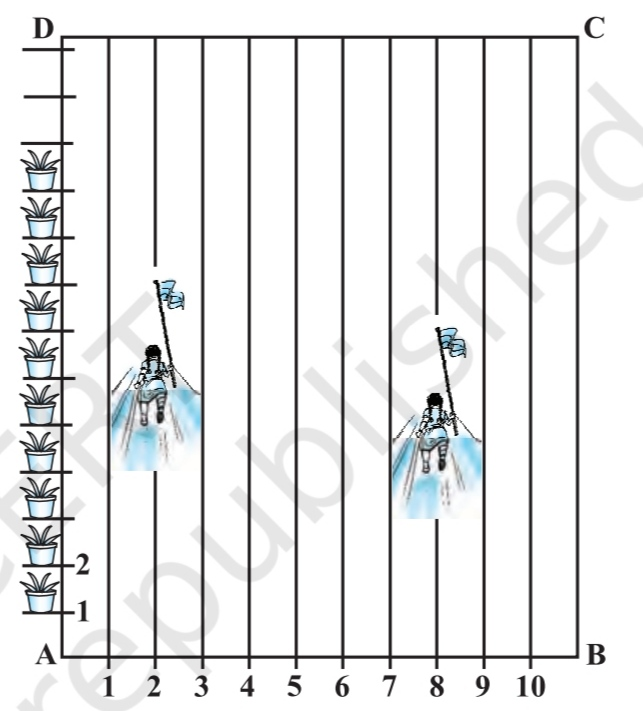
\includegraphics[width=\columnwidth]{chapters/10/figs/7.12.png}
\caption{7.12}
  \label{fig:7.12}
\end{figure}
\item Find the ratio in which the line segment joining the points $(-3,10)$ and $(6,-8)$ is divided by $(1,-6)$.
\item Find the ratio in which the line segment joining $A(1,-5)$ and $B(-4,5)$ is divided by the x-axis. Also find the coordinates of the point of division.
\item If $(1,2), (4,y), (x,6)$ and $(3,5)$ are the vertices of parallelogram taken in order, find x and y.
\item Find the coordinates of a point A, where AB is the diameter of a circle whose centre is $(2,-3)$ and B is $(1,4)$.
\item If A and B are $(-2,-2)$ and $(2,-4)$ respectively, find the coordinates of P such that AP= $\frac {3}{7}$ AB  and P lies on the line segment AB.
\item Find the coordinates of the points which divide the line segment joining A $(2,-2)$ and B $(2,8)$ into four equal parts.
\item Find the area of a rhombus if its vertices are $(3,0), (4,5), (1,-4)$ and $(-2,-1)$ taken in order.
\end{enumerate}
